\documentclass[tikz,border=8pt]{standalone}
\usetikzlibrary{arrows.meta,patterns}
\definecolor{bg}{HTML}{FAFAF7}
\definecolor{steel}{HTML}{8D99A6}
\definecolor{steeldark}{HTML}{4E5A66}
\definecolor{steellight}{HTML}{C9D1D9}
\definecolor{oilhi}{HTML}{E8A33D}
\definecolor{oillo}{HTML}{F6DDA6}
\definecolor{seal}{HTML}{2F2F2F}
\definecolor{label}{HTML}{233044}
\definecolor{arrowhi}{HTML}{D1495B}
\definecolor{arrowlo}{HTML}{3F7CAC}
\begin{document}
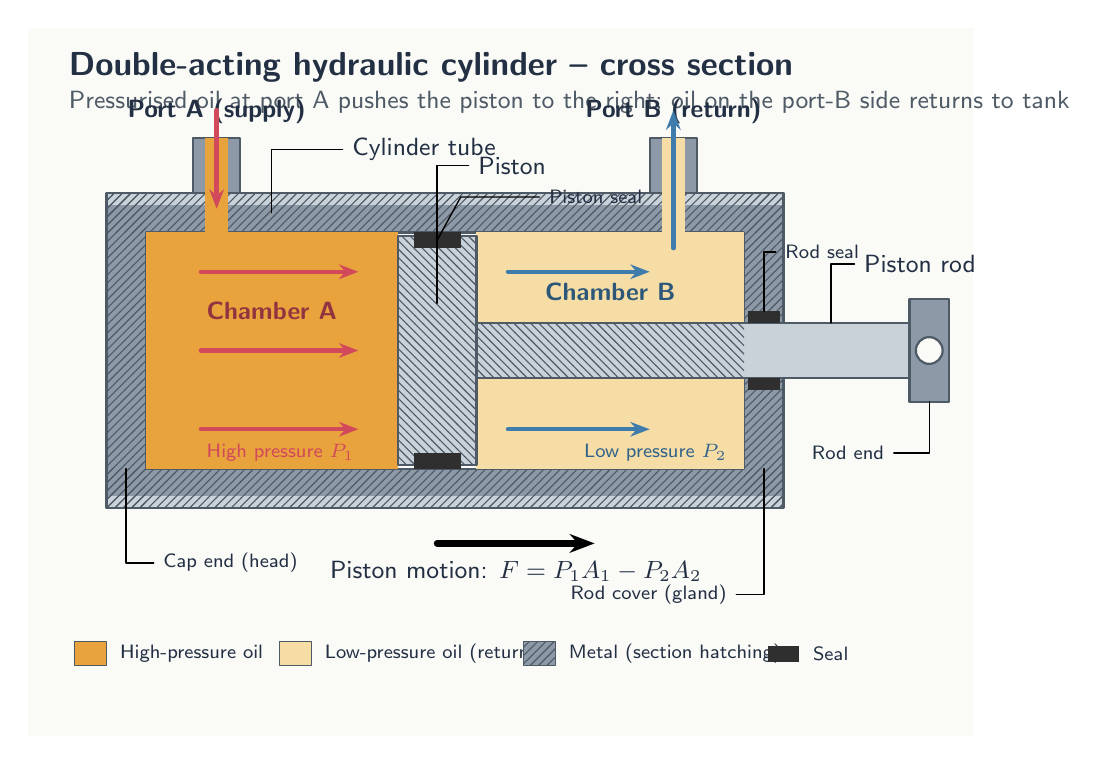
\begin{tikzpicture}[x=1cm,y=1cm,line join=round,line cap=round,
  lbl/.style={font=\sffamily\small,text=label},
  ttl/.style={font=\sffamily\bfseries\large,text=label},
  lead/.style={label,line width=0.5pt},
  flow/.style={-{Stealth[length=7pt]},line width=1.6pt}]
  \fill[bg] (-0.6,-0.9) rectangle (11.4,8.1);
  \node[ttl,anchor=west] at (-0.2,7.6) {Double-acting hydraulic cylinder -- cross section};
  \node[lbl,anchor=west,text=steeldark] at (-0.2,7.15) {Pressurised oil at port A pushes the piston to the right; oil on the port-B side returns to tank};

  % ===== cylinder body (section) =====
  \fill[steel] (0.4,2.0) rectangle (9.0,2.5);   % bottom wall
  \fill[steel] (0.4,5.5) rectangle (9.0,6.0);   % top wall
  \fill[steel] (0.4,2.0) rectangle (0.9,6.0);   % left cap
  \fill[steel] (8.5,2.0) rectangle (9.0,6.0);   % right cap (with rod gland)
  \fill[steellight] (0.4,5.85) rectangle (9.0,6.0);
  \fill[steellight] (0.4,2.0) rectangle (9.0,2.15);
  \draw[steeldark,line width=0.8pt] (0.4,2.0) rectangle (9.0,6.0);
  \draw[steeldark,line width=0.8pt] (0.9,2.5) rectangle (8.5,5.5);
  % hatching to mark the cut metal
  \fill[pattern=north east lines,pattern color=steeldark] (0.4,2.0) rectangle (9.0,2.5);
  \fill[pattern=north east lines,pattern color=steeldark] (0.4,5.5) rectangle (9.0,6.0);
  \fill[pattern=north east lines,pattern color=steeldark] (0.4,2.0) rectangle (0.9,6.0);
  \fill[pattern=north east lines,pattern color=steeldark] (8.5,2.0) rectangle (9.0,6.0);

  % ===== chambers =====
  % cap side (left, high pressure)
  \fill[oilhi] (0.9,2.5) rectangle (4.1,5.5);
  % rod side (right, low pressure, annular around the rod)
  \fill[oillo] (5.1,2.5) rectangle (8.5,5.5);

  % ===== piston + rod =====
  \fill[steellight,draw=steeldark,line width=0.8pt] (4.1,2.55) rectangle (5.1,5.45);
  \fill[pattern=north west lines,pattern color=steeldark] (4.1,2.55) rectangle (5.1,5.45);
  % piston seals (o-rings) top & bottom
  \fill[seal] (4.3,5.3) rectangle (4.9,5.5);
  \fill[seal] (4.3,2.5) rectangle (4.9,2.7);
  % rod
  \fill[steellight,draw=steeldark,line width=0.8pt] (5.1,3.65) rectangle (10.6,4.35);
  \fill[pattern=north west lines,pattern color=steeldark] (5.1,3.65) rectangle (8.5,4.35);
  \draw[steeldark,line width=0.5pt] (8.5,3.65) -- (10.6,3.65) (8.5,4.35) -- (10.6,4.35);
  % rod gland seal + wiper on the right cap
  \fill[seal] (8.55,4.35) rectangle (8.95,4.5);
  \fill[seal] (8.55,3.5) rectangle (8.95,3.65);
  % rod eye at the end
  \fill[steel,draw=steeldark,line width=0.8pt] (10.6,3.35) rectangle (11.1,4.65);
  \fill[bg,draw=steeldark,line width=0.8pt] (10.85,4.0) circle (0.17);

  % ===== ports =====
  \fill[steel,draw=steeldark,line width=0.8pt] (1.5,6.0) rectangle (2.1,6.7);
  \fill[oilhi] (1.65,5.5) rectangle (1.95,6.7);
  \fill[steel,draw=steeldark,line width=0.8pt] (7.3,6.0) rectangle (7.9,6.7);
  \fill[oillo] (7.45,5.5) rectangle (7.75,6.7);
  \node[lbl,anchor=south,font=\sffamily\bfseries\small] at (1.8,6.75) {Port A (supply)};
  \node[lbl,anchor=south,font=\sffamily\bfseries\small] at (7.6,6.75) {Port B (return)};

  % ===== fluid flow arrows =====
  \draw[flow,arrowhi] (1.8,7.05) -- (1.8,5.8);
  \foreach \y in {3.0,4.0,5.0}{
    \draw[flow,arrowhi] (1.6,\y) -- (3.6,\y);
  }
  \foreach \y in {3.0,5.0}{
    \draw[flow,arrowlo] (5.5,\y) -- (7.3,\y);
  }
  \draw[flow,arrowlo] (7.6,5.3) -- (7.6,7.05);
  \node[lbl,text=arrowhi,font=\sffamily\scriptsize,anchor=west] at (1.55,2.7) {High pressure $P_1$};
  \node[lbl,text=arrowlo!80!black,font=\sffamily\scriptsize,anchor=east] at (8.4,2.7) {Low pressure $P_2$};

  % piston motion arrow
  \draw[-{Stealth[length=9pt]},line width=2.4pt,label] (4.6,1.55) -- (6.6,1.55);
  \node[lbl,anchor=north] at (5.6,1.45) {Piston motion: $F = P_1 A_1 - P_2 A_2$};

  % ===== labels with leader lines =====
  \draw[lead] (2.5,5.75) -- (2.5,6.55) -- (3.4,6.55);
  \node[lbl,anchor=west] at (3.4,6.55) {Cylinder tube};
  \draw[lead] (4.6,4.6) -- (4.6,6.35) -- (5.0,6.35);
  \node[lbl,anchor=west] at (5.0,6.35) {Piston};
  \draw[lead] (4.6,5.4) -- (4.9,5.95) -- (5.9,5.95);
  \node[lbl,anchor=west,font=\sffamily\scriptsize] at (5.9,5.95) {Piston seal};
  \draw[lead] (9.6,4.35) -- (9.6,5.1) -- (9.9,5.1);
  \node[lbl,anchor=west] at (9.9,5.1) {Piston rod};
  \draw[lead] (8.75,4.5) -- (8.75,5.25) -- (8.9,5.25);
  \node[lbl,anchor=west,font=\sffamily\scriptsize] at (8.9,5.25) {Rod seal};
  \draw[lead] (10.85,3.35) -- (10.85,2.7) -- (10.4,2.7);
  \node[lbl,anchor=east,font=\sffamily\scriptsize] at (10.4,2.7) {Rod end};
  \draw[lead] (0.65,2.5) -- (0.65,1.3) -- (1.0,1.3);
  \node[lbl,anchor=west,font=\sffamily\scriptsize] at (1.0,1.3) {Cap end (head)};
  \draw[lead] (8.75,2.5) -- (8.75,0.9) -- (8.4,0.9);
  \node[lbl,anchor=east,font=\sffamily\scriptsize] at (8.4,0.9) {Rod cover (gland)};
  \node[lbl,anchor=center,text=arrowhi!70!black,font=\sffamily\bfseries\small] at (2.5,4.5) {Chamber A};
  \node[lbl,anchor=center,text=arrowlo!70!black,font=\sffamily\bfseries\small] at (6.8,4.75) {Chamber B};

  % ===== legend =====
  \fill[oilhi,draw=steeldark,line width=0.4pt] (0.0,0.0) rectangle (0.4,0.3);
  \node[lbl,anchor=west,font=\sffamily\scriptsize] at (0.45,0.15) {High-pressure oil};
  \fill[oillo,draw=steeldark,line width=0.4pt] (2.6,0.0) rectangle (3.0,0.3);
  \node[lbl,anchor=west,font=\sffamily\scriptsize] at (3.05,0.15) {Low-pressure oil (return)};
  \fill[steel,draw=steeldark,line width=0.4pt] (5.7,0.0) rectangle (6.1,0.3);
  \fill[pattern=north east lines,pattern color=steeldark] (5.7,0.0) rectangle (6.1,0.3);
  \node[lbl,anchor=west,font=\sffamily\scriptsize] at (6.15,0.15) {Metal (section hatching)};
  \fill[seal] (8.8,0.05) rectangle (9.2,0.25);
  \node[lbl,anchor=west,font=\sffamily\scriptsize] at (9.25,0.15) {Seal};
\end{tikzpicture}
\end{document}
